\documentclass{article}

\usepackage[version=3]{mhchem} % Package for chemical equation typesetting
\usepackage{siunitx} % Provides the \SI{}{} and \si{} command for typesetting SI units
\usepackage{graphicx} % Required for the inclusion of images
\usepackage{natbib} % Required to change bibliography style to APA
\usepackage{amsmath} % Required for some math elements 
\usepackage{listings}
\usepackage{graphicx}


\setlength\parindent{0pt} % Removes all indentation from paragraphs

\renewcommand{\labelenumi}{\alph{enumi}.} % Make numbering in the enumerate environment by letter rather than number (e.g. section 6)

%\usepackage{times} % Uncomment to use the Times New Roman font

%----------------------------------------------------------------------------------------
%	DOCUMENT INFORMATION
%----------------------------------------------------------------------------------------

\title{COMPTE RENDU TP 1\footnote{Le code est en libre accès sur \url{https://github.com/GuiMarion/SignalProcessing}} \\ Introduction à MatLab et exemples loupe spectrale} % Title

\author{Guilhem \textsc{MARION} et Clément \textsc{LE MOINE VEILLON}} % Author name



\date{\today} % Date for the report

\begin{document}

\maketitle

\section{premier.m}



\paragraph{}
Si x et h ont pour longueurs respectives $N$ et $M$ alors le produit de convolution est de taille $N+M-1$ et s'écrit pour tout n tel que  $0 \leq n \leq N + M-2$ : 

\begin{center}\ce{$y(n) = \sum_{m=0}^{N+M-2} x(m) h(n-m)$}\end{center}

\paragraph{}
L'idée est de rajouter des zéros à x et h pour que tout se passe bien lors du produit de convolution que l'on transcrit en un produit scalaire par blocs. 

\paragraph{remarque :}
N'est ajouté au compte rendu que le code jugé pertinent à la compréhension du TP, les redites notamment dans les classes sont évitées.

\paragraph{}
On définit une classe $functionx$ associée au vecteur $x$ avec notamment des méthodes pour obtenir et afficher une partie du signal échantillonné définie entre les rangs $i_{min}$ et $i_{max}$ : 
$\\ $
\begin{lstlisting}
class functionX:

   def __init__(self, N):
        self.N = N
        self.X = []
        for i in range(N):
            self.X.append(i+1)

    def __str__(self):
        return str(self.X)


    def plot(self):
        plt.plot(self.X)
        plt.show()


    def getElem(self,i):
        if i < self.N and i >= 0:
            return self.X[i]

        else :
            return 0

    def getElems(self, imin, imax):

        if imax < self.N:
            return self.X[imin:imax]
        else:
            return self.X[imin : self.N] + [0]*(imax-self.N)
        

    def getAllValues(self):
        return self.X

    def getSize(self):
        return self.N

    def printSignal(self, imin, imax):
        print(self.getElems(imin,imax))

\end{lstlisting}

$\\ $


De même on définit une classe $functionH$ associée au vecteur $h$ dans le même esprit que $functionX$ :

$\\$

\begin{lstlisting}
class functionH:

def __init__(self, N):
        self.N = N
        self.X = []
        for i in range(N):
            self.X.append(1)

\end{lstlisting}

$\\$

On peut ensuite définir une fonction de convolution $conv$ qui prend en entrée $x$ et $h$ de tailles quelconques et renvoie la convolution entre les deux : 

\begin{lstlisting}
def conv(x, h):

time_start = time.clock()
    Max = max(x.getSize(), h.getSize())

    Y = []

    for n in range(Max):

        ret = 0
        for i in range(2*Max):
            ret += h.getElem(i)*x.getElem(n-i)

        Y.append(ret)

    time_elapsed = (time.clock() - time_start)
    print()
    print("Computation time:",time_elapsed)
    print()

    return Y
\end{lstlisting}

\paragraph{Application : }

On crée une rampe bruitée de 100 points que l'on va lisser en utilisant un RIF moyenneur.

$\\ $

On définit une classe $functionXNoisy$ sur le modèle de $functionX$ mais en intégrant un bruit aléatoire centré en $0$ dont le niveau est règlable par le paramètre $B$ : 
$\\$
\begin{lstlisting}
class functionXNoisy:

    # B niveau de bruit
    def __init__(self, N, B):
        self.N = N
        self.X = []
        for i in range(N):
            self.X.append(i+1 - random.random()*B +0.5)

   

\end{lstlisting}
$\\  $
On définit également une classe $functionHN$ associée à filtre moyenneur dont les $N$ éléments valent $\frac{1}{N}$ :
$\\ $
\begin{lstlisting}
class functionHN:

    def __init__(self, N):
        self.N = N
        self.X = []
        for i in range(N):
            self.X.append(1/N)

   

 
\end{lstlisting}


$\\ $
Il est aisé de calculer ensuite la convolution entre le filtre moyenneur $HN$ et le signal bruité $XNoisy$ en jouant sur $M$ l'ordre du filtre (On choisit $M = 30$ ici), puis de l'afficher :
\\ 
\begin{lstlisting}
x = functionXNoisy(10, 1)
h = functionHN(30)

Y = conv(x,h)

plt.plot(Y, 'k')
plt.plot([x.getElem(i) for i in range(30)])
plt.show()
\end{lstlisting}

On peut alors afficher le résultat de la convolution en noir et le signal d'entrée en bleu pour différentes valeurs de $M$ 50, 100, 150.

\begin{figure}[!ht]
    \center
    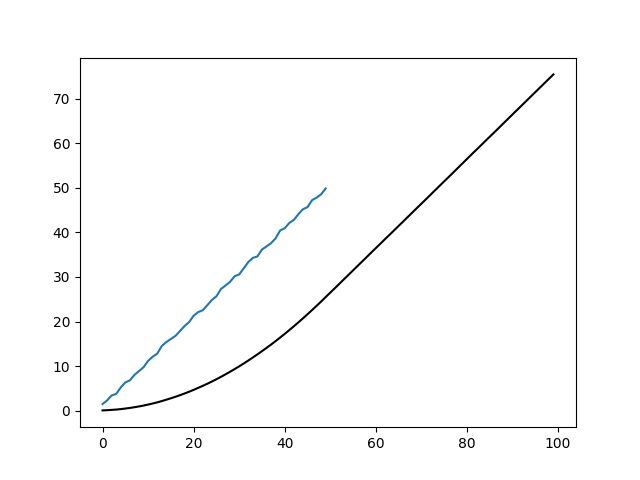
\includegraphics[width=10cm]{Premier_100_50.png}
    \caption{Y et x pour M=50}
\end{figure}

\begin{figure}[!ht]
    \center
    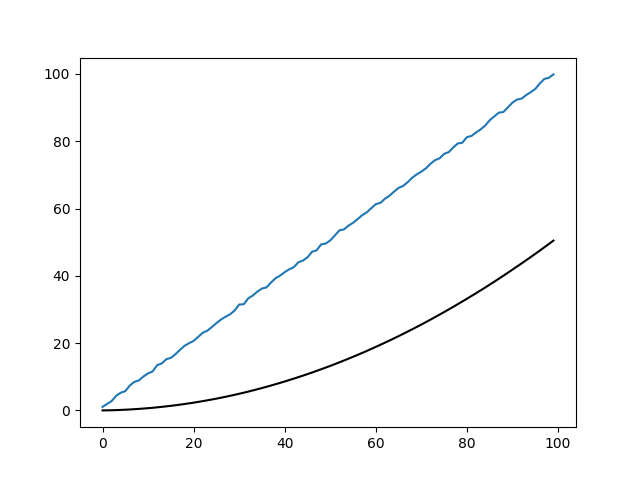
\includegraphics[width=10cm]{Premier_100_100.png}
    \caption{Y et x pour M=100}
\end{figure}

\begin{figure}[!ht]
    \center
    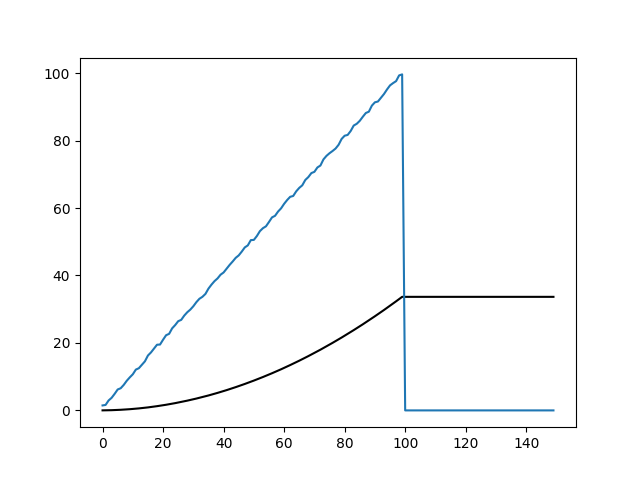
\includegraphics[width=10cm]{Premier_100_150.png}
    \caption{Y et x pour M=150}
\end{figure}

\section{Affichage d'un sinus - Stroboscopie}

On va créer une classe $Sinus$ en commençant par définir le $sinus$ lui même : 
$\\ $
\begin{lstlisting}
def __init__(self, N, nu0):

        self.N = N
        self.nu0 = nu0
        self.SIN = []
        for i in range(self.N):
            self.SIN.append(math.sin(2*math.pi*self.nu0*i))

\end{lstlisting}
$\\ $
On définit une manière de le représenter :
$\\ $
\begin{lstlisting}
def plot(self):
        plt.plot(self.SIN)
        plt.show()
\end{lstlisting}
$\\ $
On définit une manière interactive d'obtenir les valeurs du $sinus$ entre  $n_{min}$ et $n_{max}$, ainsi que la taille de son support :
$\\ $
\begin{lstlisting}
def getValues(self,nMin, nMax):

        return self.SIN[nMin : nMax]

    def getAllValues(self):

        return self.SIN

    def getSize(self):
        return self.N
\end{lstlisting}
$\\ $
On définit une manière de représenter sa $TF$ :
$\\ $
\begin{lstlisting}
def plotFFT(self):


        t = np.arange(self.N)
        sp = np.fft.fft(self.SIN)
        freq = np.fft.fftfreq(t.shape[-1])
        plt.plot(freq, sp.real, freq, sp.imag)
        
        plt.show()  
\end{lstlisting}



\paragraph{Cas $\nu_{0} = 0.49$ : }


\begin{figure}[h!]
    \begin{minipage}[c]{.46\linewidth}
        \centering
        \includegraphics[width=7cm]{sinus_049.png}
        \caption{sinus de fréquence réduite 0.49}
    \end{minipage}
    \hfill%
    \begin{minipage}[c]{.46\linewidth}
        \centering
        \includegraphics[width=7cm]{sinus_001.png}
        \caption{sinus de fréquence réduite 0.01}
    \end{minipage}
\end{figure}


$\\ \\$
En temporel, on observe un effet d'optique, le sinus parait modulé en amplitude (enveloppe) mais il n'est n'en est rien, c'est l'échantillonnage qui produit cet effet.
\\ \\
En fréquentiel, on ne voit pas la raie à la fréquence $\nu_{0}$ car l'échantillonnage ne le permet pas,  il y a trop peu d'échantillons. 

\paragraph{Variation de $\nu_{0}$ : }
Plus $\nu_{0}$ est petit plus l'échantillonnage est précis.


\paragraph{Remarque : }
On ne sait pas vraiment quel signal on observe, en effet $\nu_{0}= \frac{f}{f_{e}}$ donc à $\nu_{0}$ fixé il y a une infinité de valeurs de $f$ et de $f_{e}$ et donc une infinité de sigaux sinusoïdaux possibles si on fixe la fréquence d'échantillonnage et d'échantillonnages possibles si on fixe la fréquence du sinus.
$\\ \\$


\section{Observation du spectre par la TFD}

On créé une classe $Cosinus$ :

\begin{lstlisting}
class Cosinus:

    def __init__(self, N, nu0):

        self.N = N
        self.nu0 = nu0
        self.COS = []
        for i in range(self.N):
            self.COS.append(math.cos(2*math.pi*self.nu0*i))
\end{lstlisting}

$\\$

On défini une fonction $Obspec$ au sein de la classe $Cosinus$ qui va nous permettre d'observer le spectre d'un $cosinus$ :

$\\$

\begin{lstlisting}
def obspec(self, H, Nfft, nu0):

        Y = mult(self.COS, H.getAllValues())

        t = np.arange(Nfft)
        sp = np.fft.fft(Y, n = Nfft)
        freq = np.fft.fftfreq(Nfft)

        Y = []

        for i in range(len(sp.real)):
            Y.append(20*math.log10(math.sqrt(sp.real[i]**2 + sp.imag[i]**2)))

        plt.plot(freq, Y)    
    
        plt.show() 
\end{lstlisting}


\subsection{Application pour $\nu_{0}=0.1, 0.125, N=64$ avec une fenêtre rectangulaire et pour les valeurs  $Nfft=32, 64, 128, 1024$}




\begin{figure}[h!]
    \begin{minipage}[c]{.46\linewidth}
        \centering
        \includegraphics[width=7cm]{TFD-32-01-BoxCar}
        \caption{TFD pour $N=32, \nu_{0}=0.1$}
    \end{minipage}
    \hfill%
    \begin{minipage}[c]{.46\linewidth}
        \centering
        \includegraphics[width=7cm]{TFD-32-0125-BoxCar}
        \caption{TFD pour $N=32, \nu_{0}=0.125$}
    \end{minipage}
\end{figure}

\begin{figure}[h!]
    \begin{minipage}[c]{.46\linewidth}
        \centering
        \includegraphics[width=7cm]{TFD-64-01-BoxCar.png}
        \caption{TFD pour $N=64, \nu_{0}=0.1$}
    \end{minipage}
    \hfill%
    \begin{minipage}[c]{.46\linewidth}
        \centering
        \includegraphics[width=7cm]{TFD-64-0125-BoxCar}
        \caption{TFD pour $N=64, \nu_{0}=0.125$}
    \end{minipage}
\end{figure}

\begin{figure}[h!]
    \begin{minipage}[c]{.46\linewidth}
        \centering
        \includegraphics[width=7cm]{TFD-128-01-BoxCar.png}
        \caption{TFD pour $N=128, \nu_{0}=0.1$}
    \end{minipage}
    \hfill%
    \begin{minipage}[c]{.46\linewidth}
        \centering
        \includegraphics[width=7cm]{TFD-128-0125-BoxCar}
        \caption{TFD pour $N=128, \nu_{0}=0.125$}
    \end{minipage}
\end{figure}

\begin{figure}[h!]
    \begin{minipage}[c]{.46\linewidth}
        \centering
        \includegraphics[width=7cm]{TFD-1024-01-BoxCar.png}
        \caption{TFD pour $N=1024, \nu_{0}=0.1$}
    \end{minipage}
    \hfill%
    \begin{minipage}[c]{.46\linewidth}
        \centering
        \includegraphics[width=7cm]{TFD-1024-0125-BoxCar}
        \caption{TFD pour $N=1024, \nu_{0}=0.125$}
    \end{minipage}
\end{figure}
$\\$

$\\$
$\\$
$\\$
$\\$
$\\$
$\\$$\\$$\\$$\\$
$\\$
$\\$

\subsection{Application pour $\nu_{0}=0.1, 0.125, N=64$ avec les fenêtres rectangulaire et Hanning pour   $Nfft=1024$}

\begin{figure}[h!]
    \begin{minipage}[c]{.46\linewidth}
        \centering
        \includegraphics[width=7cm]{TFD-1024-01-BoxCar.png}
        \caption{TFD pour $N=1024$ fenêtre rectangulaire}
    \end{minipage}
    \hfill%
    \begin{minipage}[c]{.46\linewidth}
        \centering
        \includegraphics[width=7cm]{TFD-1024-01-Hanning}
        \caption{TFD pour $N=1024$ fenêtre de Hanning}
    \end{minipage}
\end{figure}

On constate que pour Hanning les lobes secondaires sont largement atténués par rapport au cas fenêtre rectangulaire, la contrepartie c'est que les deux pics sont moins précis (plus larges) et atténués. En fontion de ce qu'on voudra observer, l'usage de l'une ou l'autre de ces fenêtres sera plus adapté.

\section{Réalisation d'une loupe spectrale}
\subsection{Principe de traitement}
$x_{n}=\cos(2\pi\nu_{0}n+\beta\sin(2\pi\nu_{m}n))$

On définit d'abord une classe $W_{1}$ :

\begin{lstlisting}
class W1:

    def __init__(self, N, nu0):
        self.N = N
        self.X = []

        for i in range(N):
            self.X.append(cmath.exp(2j * math.pi * nu0*i))


        self.name = "W1"
\end{lstlisting}

On définit ensuite une classe $Func$ qui accueillera toutes les opérations nécessaires à chaque étape, on  définit notamment $Multiply$ : 

\begin{lstlisting}
def Multiply(X, W):

    Y = []

    for i in range(X.getSize()):

        Y.append(X.getElem(i)*W.getElem(i))

    return Y
\end{lstlisting}

Le code pour l'étape 1 est le suivant :
\begin{lstlisting}
    w1 = W1(N, nu0)
    X1 = Func(Multiply(X, w1))
    X1.plotFFT()
\end{lstlisting}

Le code pour l'étape 2 est le suivant :
\begin{lstlisting}
   H = BoxCar(N//2)
   X2 = Func(conv(X1, H))
   X2.plotFFT()
\end{lstlisting}

Pour l'étape 3 on rajoute une méthode $Decimate$ dans $Func$ :
\begin{lstlisting}
   def Decimate(X, M):

    Y = []

    mX = X.getAllValues()

    for i in range(X.getSize()//M):
        Y.append(mX[i*M])

    return Y
\end{lstlisting}

Le code pour l'étape 3 est le suivant :
\begin{lstlisting}
   X3 = Func(Decimate(X2,10))
   X3.plotFFT()
\end{lstlisting}

Le code pour l'étape 4 est le suivant :
\begin{lstlisting}
   w2 = W1(N, -0.5)
   Y1 = Func(Multiply(X3, w2))
   Y1.plotFFT()
\end{lstlisting}

A l'étape 5, on fait simplement une TFD pour obtenir le spectre.

\subsection{Développement et programmation}

\paragraph{Compréhension :}

$\ $
\begin{figure}[h!]
    \begin{minipage}[c]{.46\linewidth}
        \centering
        \includegraphics[width=7cm]{51-X1.png}
        \caption{TFD de $x_{1}$}
    \end{minipage}
    \hfill%
    \begin{minipage}[c]{.46\linewidth}
        \centering
        \includegraphics[width=7cm]{51-X2}
        \caption{TFD de $x_{2}$}
    \end{minipage}
\end{figure}

\begin{figure}[h!]
    \begin{minipage}[c]{.46\linewidth}
        \centering
        \includegraphics[width=7cm]{51-X3}
        \caption{TFD pour $x_{3}$}
    \end{minipage}
    \hfill%
    \begin{minipage}[c]{.46\linewidth}
        \centering
        \includegraphics[width=7cm]{51-Y1}
        \caption{TFD de $y$}
    \end{minipage}
\end{figure}




Valeur maximale de M : 
\begin{align*}
M &\leq \frac{1}{\Delta\nu} \\
M &\leq \frac{1}{3*(10+1)*5*10^{-4}} \\
M &\leq 32
\end{align*}

$ \ $

%\paragraph{Zoom rudimentaire}

\begin{figure}[!h]
    \center
    \includegraphics[width=7cm]{52-X4}
    \caption{TFD d'ordre $MN$ de $x$ avec fenêtre de Hanning}
\end{figure}
$\\\\\\\\\\\\\\\\\\$
Il manque la figure du zoom rudimentaire mais ce qu'on voit est une oscillation, comme si le pic était bruité.
$\\\\$

\paragraph{Synthèse du filtre}

\begin{figure}[!h]
    \center
    \includegraphics[width=7cm]{52-HanningX(NM)}
    \caption{TFD d'ordre $MN$ de $x_{1}$ avec fenêtre de Hanning}
\end{figure}

Ici on filtre $x_{1}$ à l’aide de l’algorithme d’échange
de Remez, observons les spectres :

\begin{figure}[h!]
    \begin{minipage}[c]{.46\linewidth}
        \centering
        \includegraphics[width=7cm]{52-RemezBoxcar}
        \caption{TFD pour $x_{2}$ en fenêtre rectangulaire }
    \end{minipage}
    \hfill%
    \begin{minipage}[c]{.46\linewidth}
        \centering
        \includegraphics[width=7cm]{52-RemezHanning}
        \caption{TFD pour $x_{2}$ en fenêtre Hanning}
    \end{minipage}
\end{figure}

$\\\\\\$
On cherche des valeurs de $\nu_{a}$ et $\nu_{c}$ pour limiter l'ordre du filtre, Il faut $\nu_{a} - \nu_{c}$ le plus grand possible tout en filtrant la bonne chose, graphiquement on trouve $\nu_{a}=0.3$ et $\nu_{c}=0.06$. De même pour obtenir une grosse atténuation on prend $\delta_{1} = 0.1$ et $\delta_{1} = 1/100000000$.



$\\\\\\\  $

\paragraph{Dernières étapes}


\begin{figure}[h!]
    \begin{minipage}[c]{.46\linewidth}
        \center
        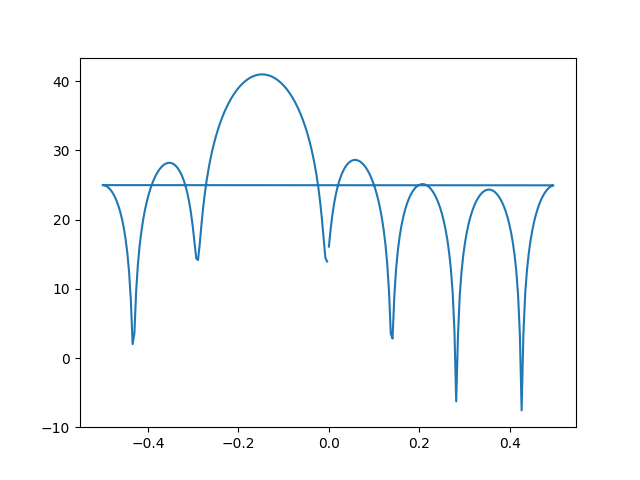
\includegraphics[width=7cm]{Loupe.png}
        \caption{Loupe spectrale}
    \end{minipage}
    \hfill%
    \begin{minipage}[c]{.46\linewidth}
        \center
        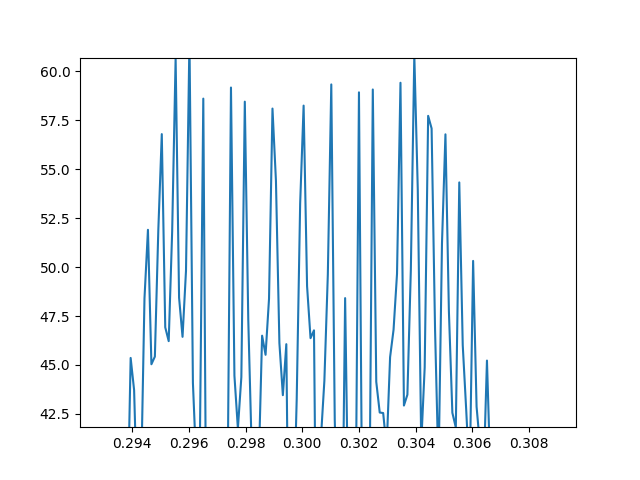
\includegraphics[width=7cm]{pic.png}
        \caption{Zoom}
    \end{minipage}
\end{figure}





